% Options for packages loaded elsewhere
%\PassOptionsToPackage{unicode}{hyperref}
%\PassOptionsToPackage{hyphens}{url}
%\PassOptionsToPackage{dvipsnames,svgnames,x11names}{xcolor}
%
\documentclass[doc,a4paper]{apa7}
\usepackage[utf8]{inputenc}
\usepackage[T1]{fontenc}
\usepackage[style=apa, backend=biber]{biblatex}
\usepackage{booktabs}
\usepackage{longtable}
% \usepackage{amsmath,amssymb}
% \usepackage{setspace}
\usepackage{graphicx}
\usepackage[export]{adjustbox}
% \usepackage{color}
\usepackage{xcolor}
\usepackage{array}
\usepackage{calc} % for calculating minipage widths
\usepackage{etoolbox}
\makeatletter
\patchcmd\longtable{\par}{\if@noskipsec\mbox{}\fi\par}{}{}
\makeatother
% Allow footnotes in longtable head/foot
\IfFileExists{footnotehyper.sty}{\usepackage{footnotehyper}}{\usepackage{footnote}}
\makesavenoteenv{longtable}
\setlength{\emergencystretch}{3em} % prevent overfull lines
\providecommand{\tightlist}{%
  \setlength{\itemsep}{0pt}\setlength{\parskip}{0pt}}
\setcounter{secnumdepth}{-\maxdimen} % remove section numbering
\ifLuaTeX
  \usepackage{selnolig}  % disable illegal ligatures
\fi
\usepackage{bookmark}
\IfFileExists{xurl.sty}{\usepackage{xurl}}{} % add URL line breaks if available
\urlstyle{same}
\hypersetup{
  colorlinks=true,
  linkcolor={blue},
  filecolor={Maroon},
  citecolor={blue},
  urlcolor={blue},
  pdfcreator={Christophe Pallier <christophe@pallier.org>}}

% --------------------------- Content -----------------------------------------------------------------

\title{Goxpyriment: A Go Framework for Behavioral and Cognitive Experiments}
\shorttitle{Let's go experiment!}

\authorsnames{Christophe Pallier, Julie Bonnaire, Marie-France Fourcade}
\authorsaffiliations{Cognitive Neuroimaging Unit, CNRS INSERM CEA}

\authornote{\addORCIDlink{Christophe Pallier}{0000-0002-3324-666X} Correspondence should be addressed to  C. Pallier, Cognitive Neuroimaging Unit, Neurospin, Gif-sur-Yvette, F-91191, France. E-mail: christophe@pallier.org. I would like to thanks Luca Bonatti and Raphael Bordas for alpha testing this software. The authors have no conflicts of interest to disclose.}

\keywords{framework, library, stimulus presentation, timing, behavioral experiments, psychophysics, psychology}

\addbibresource{biblio.bib}

\abstract{
We introduce \texttt{goxpyriment}, a new open-source software
framework for programming behavioral and cognitive experiments using
the Go programming language. The library is designed to address some
limitations of existing Python-based experiment tools, particularly
the runtime environment complexity that frequently complicates
deployment across laboratories. Because Go is a compiled language that
can natively embed assets (e.g., graphics, audio files, and stimulus
lists),
\texttt{goxpyriment} compiles entire experiments into single,
self-contained executable binaries with zero runtime dependencies. This
drastically simplifies distribution to collaborators and testing computers.
\texttt{goxpyriment} prioritizes timing
reliability. Go's garbage collector can be disabled, highly-reducing
the probability of unpredicable pauses, latencies that can ruin the
timing of the experiment. Keyboard and mouse events' timestamps at the
operating system level are available, allowing one to avoid continuous
pooling to get precise reaction times.  The programming interface,
inspired by Expyriment \parencite{krause2014}, was designed be human
friendly. The library includes an array of visual stimuli (text,
shapes, images, Gabor patches, motion clouds, ...) and audio
capabilities (WAV playback and tone generation). A set of 35 classic
psychology experiments implemented in goexpriment are provided that
promote not only learning by humans but also boost the ability of
modern AI-assisted coding tools to program experiments. Finally, a
migration guide from other frameworks is provided.  The framework is
released under the GNU General Public License v3 and is freely
available at https://github.com/chrplr/goxpyriment.}

\begin{document}
\maketitle

\subsection{Introduction}\label{introduction}

Experiment-control software occupies a central position in behavioral
and cognitive neuroscience: the temporal precision of stimulus
delivery and response recording, the ergonomics of experiment
programming, and the ease of deploying experiments to laboratory
hardware each affect the quality and reproducibility of empirical
data. Over the past two decades, Python has become the dominant
language for experiment programming, primarily through two libraries:
Expyriment \parencite{krause2014} and
PsychoPy \parencite{peirce2019}. Before Python, MATLAB with the
Psychophysics Toolbox \parencite{brainard1997, kleiner2007} was the de
facto standard in many laboratories. More recently, web-based
frameworks such as jsPsych \parencite{deleeuw2015, deleeuw2023} and
lab.js \parencite{henninger2022} have enabled large-scale online data
collection.

Each class of tool involves tradeoffs. MATLAB, with hooks to custom
written C/C++ libraries (e.g. the Psychtoolbox), offers good
timing on well-configured hardware but is proprietary and
expensive. Psychtoolbox scripts written on Windows often do not work
out of the box on Linux (and vice-versa). Python tools provide an open, flexible
programming environment with a large scientific ecosystem, but they
introduce two practical difficulties.  First, deploying an experiment
to a computer that does not already have a compatible Python
environment requires package management (conda, pip, venv) and can be
a source of breakage across operating-system versions. For example, installing
the psychopy python module under Linux often crashes while attempting to compile the wxPython
package when there is no precompiled wheel.  Second, Python's garbage
collector can introduce unpredictable pause times that corrupt the
timing of stimulus presentation and response recording during the
critical trial loop. Web-based tools trade timing precision for
accessibility: browser-mediated stimulus presentation is subject to
event-loop latency that make sub-frame timing difficult or
impossible \parencite{bridges2020, anwylirvine2021}.

The Go programming language \parencite{donovan2016} offers a different
point in the design space. It was designed for simplicity and has much
fewer moving parts than Python; as a consequence, the code tends to be
more ``boring'' (there is only one way to do things) but
predictable. Because Go is strongly typed, and favors error checking,
developping code typically requires less run-time debugging. Go compiles to native
machine code for each target platform and produces self-contained
binaries with no runtime dependencies. Its garbage collector is
concurrent and can be suspended for the duration of a timing-critical
section.  These properties make it an attractive substrate for a
behavioral experiment library that prioritizes timing reliability and
deployment simplicity.

The present article describes the design and capabilities of
\texttt{goxpyriment}, discusses its timing architecture, and situates it
relative to existing tools. Specifically, we highlight three main contributions
of this framework: (1) zero-dependency deployment via single compiled binaries
that simplify distribution across laboratory hardware; (2) native high-precision
timing achieved directly through the Go and SDL3 APIs without requiring external
C/C++ helper engines; and (3) a linear, straightforward API that is highly
suited for modern AI-assisted coding workflows.

\subsection{Core Advantages of a Compiled Framework}\label{core-advantages}

The choice of Go as the implementation language for \texttt{goxpyriment} provides
several critical advantages over the interpreted languages traditionally used in
behavioral research.

\subsubsection{Single-Binary Deployment (Zero Dependencies)}\label{single-binary-deployment}

Go compiles program into a single statically linked executable with no
external runtime dependencies. Crucially, the \texttt{go-sdl3} package
embeds the pre-built SDL3 runtime libraries \parencite{sdl3} directly into the
executable. The stimuli, experimental lists, fonts, ... can be
embedded too. As a results, distributing an experiment requires copying just one
file; there is no need to manage virtual environments, package
versions, or interpreter installations across laboratory
computers. This substantially reduces the operational overhead of
running experiments on multiple machines or sharing materials with
collaborators.

\subsubsection{Explicit Garbage Collection Control}\label{explicit-gc-control}

While the garbage collectors in languages like Python or JavaScript can
introduce unpredictable pause times that corrupt timing, Go exposes a runtime
API for suspending the garbage collector. \texttt{goxpyriment} uses this mechanism in its timing-critical loops, ensuring
that stimulus onsets and offsets are not delayed by memory management tasks.

\subsubsection{An AI-Friendly API}\label{ai-friendly-api}

Go's design emphasizes simplicity and predictability. Because the language has
few synonymous constructs and a strict type system, it is particularly
well-suited for use with AI-powered coding assistants. The linear,
straightforward API of \texttt{goxpyriment} allows researchers to leverage these
assistants to bridge gaps in their programming experience, with the Go compiler
providing a safety net by catching many common errors before the experiment is
even run.

\subsection{Timing Architecture and Precision}\label{timing-architecture}

\subsubsection{Hardware-Synchronized Presentation}\label{hardware-sync}

While many Python-based experiment frameworks achieve high-precision timing by
relying on external C/C++ engines like the Psychophysics Toolbox (PTB),
\texttt{goxpyriment} achieves equivalent low-level control directly through the
native SDL3 API \parencite{sdl3}. \texttt{screen.Update()} calls
SDL's \texttt{SDL\_RenderPresent}, which blocks until the display's
vertical retrace when VSYNC is enabled. Reliance on SDL3 also provides
the possibility to control \textit{variable refresh rate} monitors
(although the goxpyriment API itself does not currently wrap this SDL3
functionality.)

\subsubsection{High-Precision Streams}\label{high-precision-streams}

For paradigms with dense, high-speed stimulus sequences (e.g., Retinotopic stimulation),
\texttt{goxpyriment} provides specialized stream functions like
\texttt{PresentStreamOfImages}. These functions disable garbage collection,
drain the event queue, and busy-wait at the sub-frame level to ensure
that each stimulus onset is scheduled accurately. A \texttt{TimingLog}
records the target and actual onsets for post-hoc verification, as
well as the timing of keys pressed during the presentation of the
stream.

\subsubsection{Hardware-Level Response Timestamps}\label{hardware-timestamps}

Response timing in \texttt{goxpyriment} leverages SDL3 hardware event
timestamps. The \texttt{WaitKeysEventRT} method returns the
\texttt{KeyboardEvent.Timestamp} field, which is populated by the OS input
subsystem at hardware-interrupt time (nanoseconds since SDL initialization). By
comparing this with the \texttt{Screen.FlipNS()} timestamp—which uses the same
clock—reaction times can be measured with minimal jitter and no interpreter
overhead. This unified timing regime is abstracted through the
\texttt{ResponseDevice} interface, which explicitly signals whether a timestamp
is ``precise'' (hardware-level) or ``non-precise'' (polling-based).

\subsubsection{The Timing Verification Suite}\label{timing-verification}

The repository includes a dedicated timing verification suite
(\texttt{tests/Timing-Tests/}) that allows researchers to characterize
their hardware's performance. The suite includes tests for measuring
frame-interval jitter, verifying single-frame flash reliability via
photodiode, and calculating audio-visual SOA latencies. Other tests
measure hardware-buffer pipeline latency for audio and characterize
the USB-serial jitter of trigger devices. Other tests could be
implemented upon request by users to the first author.  A special
folder in goxpyriment's github repository, namely
`performance-reports`, is meant for users to share the results of tests
on their own hardware.


\subsubsection{Lifecycle and Safety}\label{lifecycle-safety}

Every experiment centers on an \texttt{Experiment} object that manages the
window, renderer, and audio subsystems. Execution is typically wrapped in a
\texttt{Run} function that provides a safety layer: if the participant presses
the Escape key or closes the window, the library catches the resulting internal
signal, safely flushes the data file to disk, and shuts down the SDL
subsystems. This ensures that data is preserved even if a session is aborted
prematurely.

\subsubsection{Defining Trials and Data Logging}\label{trials-logging}

Experiments follow a hierarchical structure of blocks and trials
directly inspired expyriment. Each trial is a
collection of factors that can be randomized and logged. Data
collection is handled by an \texttt{exp.Data} object, which writes to
a CSV file with extensive metadata headers.

\subsubsection{Pre-Experiment Setup Dialog}\label{setup-dialog}

\texttt{goxpyriment} provides an optional graphical
\texttt{GetParticipantInfo} dialog that opens before the main experiment
window (See Fig.~\ref{fig:getinfo})  It allows the experimenter to input subject
IDs, select experimental conditions from discrete menus, and toggle
settings like fullscreen mode.  These values are automatically
recorded in the output data file header.

Programs that use \texttt{GetParticipantInfo} also accept a
\texttt{-headless} command-line flag. When present, the dialog is skipped
entirely and field defaults (or values previously saved to the cache) are
used without opening any window. This is convenient for scripted or
automated runs (e.g.\ continuous integration checks or batch stimulus
generation) where interactive input is not possible.

\begin{figure}[t]
\centering
\begin{tabular}{cc}
  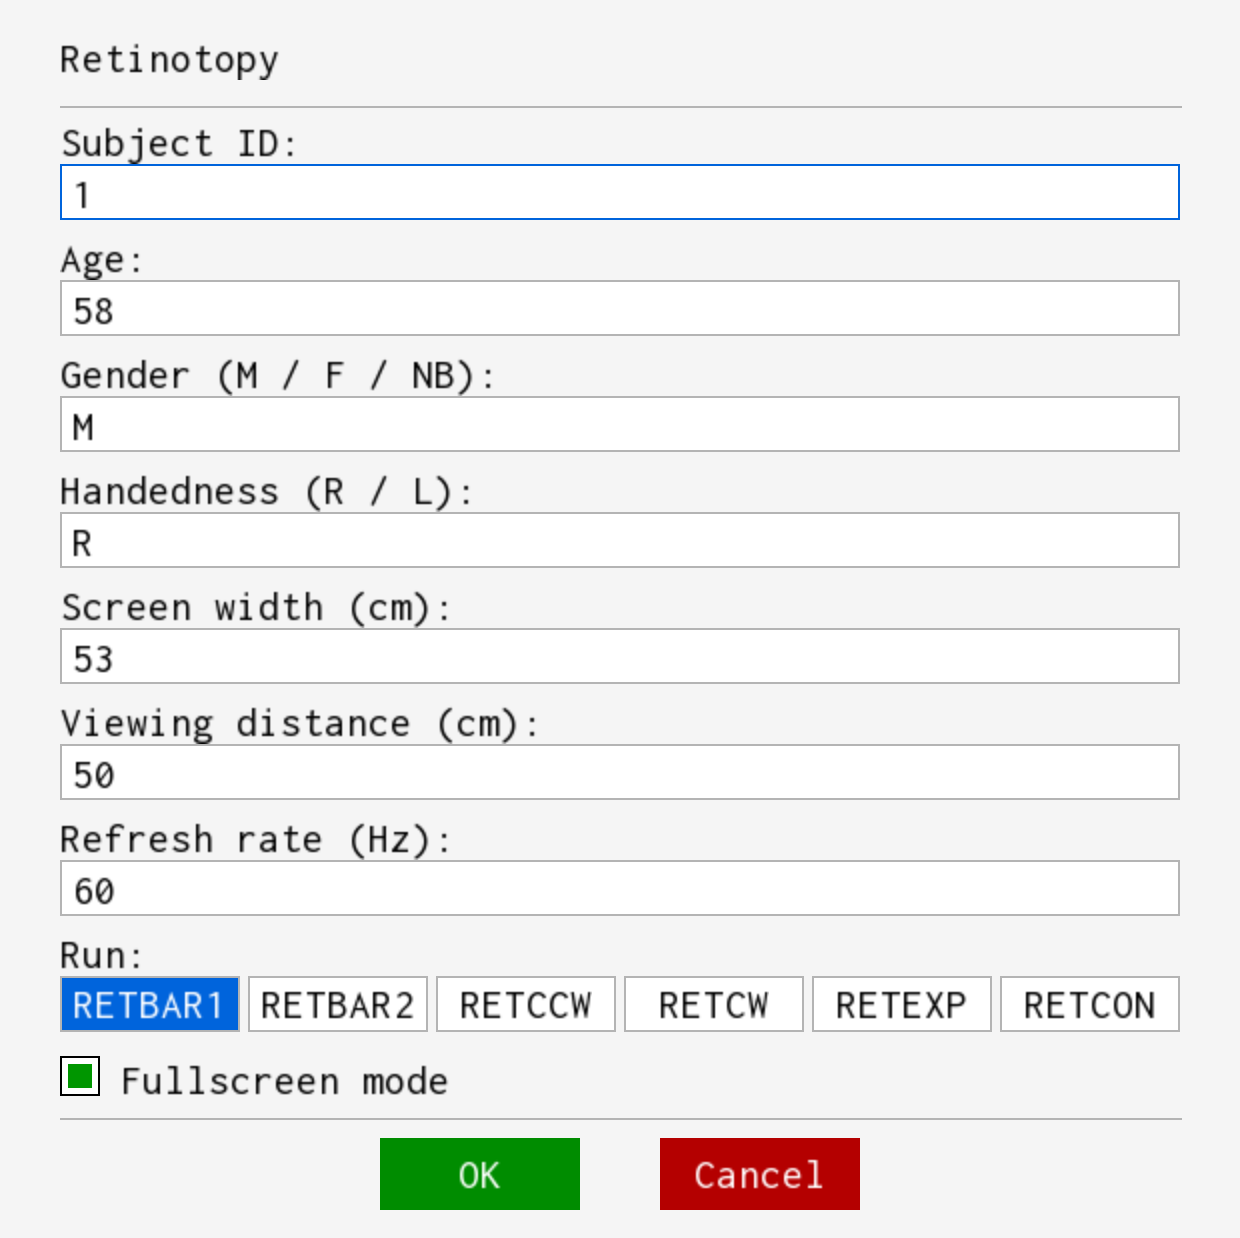
\includegraphics[width=0.5\textwidth,valign=t]{UI1.png} & 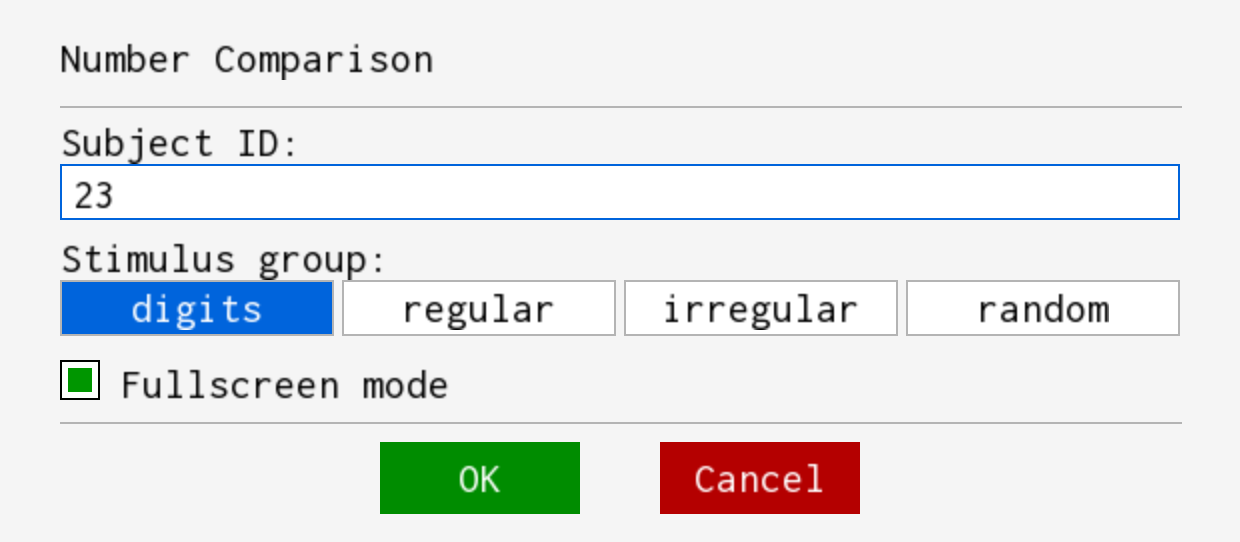
\includegraphics[width=0.5\textwidth,valign=t]{UI2.png} \\
\end{tabular}
\caption{Examples of \texttt{GetParticipantInfo} dialogs for the \emph{Retinotopy} (left) and 
\emph{Number-Comparison} (right) paradigms provided in the examples accompanying the library. These UIs makes it practical for the experimenter or participant to choose among a small fixed set of options without typing, which reduces setup errors when launching an experiment from a desktop shortcut or file manager. Note that which fields appear in the UI is configurable.}
\label{fig:getinfo}
\end{figure}


\subsection{Comparison with Existing Tools}\label{comparison-with-existing-tools}

Table 1 summarizes key properties of \texttt{goxpyriment} alongside
four widely used experiment frameworks.

\textbf{Table 1.} Comparison of selected experiment frameworks.

\begin{longtable}[]{@{}
  >{\raggedright\arraybackslash}p{(\columnwidth - 8\tabcolsep) * \real{0.2000}}
  >{\raggedright\arraybackslash}p{(\columnwidth - 8\tabcolsep) * \real{0.2000}}
  >{\raggedright\arraybackslash}p{(\columnwidth - 8\tabcolsep) * \real{0.2000}}
  >{\raggedright\arraybackslash}p{(\columnwidth - 8\tabcolsep) * \real{0.2000}}
  >{\raggedright\arraybackslash}p{(\columnwidth - 8\tabcolsep) * \real{0.2000}}@{}}
\toprule\noalign{}
\begin{minipage}[b]{\linewidth}\raggedright
Property
\end{minipage} & \begin{minipage}[b]{\linewidth}\raggedright
goxpyriment
\end{minipage} & \begin{minipage}[b]{\linewidth}\raggedright
Expyriment
\end{minipage} & \begin{minipage}[b]{\linewidth}\raggedright
PsychoPy
\end{minipage} & \begin{minipage}[b]{\linewidth}\raggedright
jsPsych
\end{minipage} \\
\midrule\noalign{}
\endhead
\bottomrule\noalign{}
\endlastfoot
Language & Go & Python & Python & JavaScript \\
Execution & Native binary & Interpreter & Interpreter & Browser \\
Deployment & Single binary & pip/conda env & Standalone app or pip &
Node.js or CDN \\
GC control & Explicit disable & No & No & No \\
VSYNC sync & Yes (SDL3) & Yes (Pygame/SDL2) & Yes (Pyglet/PTB) & Limited
(rAF) \\
Hardware triggers & Yes & Yes & Yes & No \\
Response device API & Yes & Device-specific & Device-specific & N/A \\
Event timestamp source & SDL3 hardware & Python \texttt{time.time()} & iohub or Python clock & \texttt{performance.now()} \\
Stimulus set & Moderate & Moderate & Extensive & Moderate \\
GUI builder & No & No & Yes (Builder) & No \\
Online deployment & No & No & Partial (PsychoJS) & Yes \\
Reference & This paper & \parencite{krause2014} & \parencite{peirce2019} & \parencite{deleeuw2015} \\
\end{longtable}

\texttt{goxpyriment} resembles Expyriment in its API
design: a central experiment object, a \texttt{present()}-based stimulus
API, a structured trial-loop model, and output to \texttt{.csv}-format
files with metadata. The primary technical differences are the use of Go rather than Python
and the use of SDL3 rather than the older Pygame/SDL2 stack. From the user point of view, goexpyriment adds `streams` objects which, as their name indicate, allow to display streams of stimuli, withal tightly controlled timing.  

PsychoPy offers a substantially larger stimulus set and a graphical
Builder environment; \texttt{goxpyriment} has neither of these. However,
PsychoPy's greater complexity also makes deployment and version management more
challenging. jsPsych enables large-scale online data collection, which
\texttt{goxpyriment} does not support. The MATLAB Psychophysics Toolbox (PTB)
offers the most mature timing validation in the field; \texttt{goxpyriment} aims
to achieve comparable precision through its native compiled architecture.

\subsection{Example Experiments}\label{example-experiments}

The repository provides over forty examples demonstrating classic paradigms,
including the Stroop task, Attentional Blink (RSVP), Masked Priming,
Retinotopic mapping for fMRI, and adaptive threshold estimation using the QUEST
algorithm. These examples serve as both functional templates and a gallery of
the framework's capabilities, ranging from simple parity-judgment tasks to
complex moving-dot attention studies.

\input timing-tests.tex

\subsection{Limitations and Future Directions}\label{limitations-and-future-directions}

\texttt{goxpyriment} is currently at the beta-stage, that is, the API is stabilized and we are waiting for bug reports to address them.

The current library covers the stimuli most commonly needed in cognitive psychology but does not yet
include complex 3D stimuli (which can nevertheless be programmed directly using the underlying SDL api), nor has built-in eye-tracker support. We plan to add this in a future version.

\subsection{A cautionary note about AI-assisted coding for psychologists}

As mentioned above, goexpyriment is well-suited for AI assisted coding as its API and the provided examples provide strong guidance for AI coding agents prompted to program psychology experiments. The most recent experiments in the examples gallery were actually entirely generated by Claude or Gemini (see the section Authors' contributions below. Yet, even if these agents are extremely apt and quick at coding, human supervision is still clearly necessary as exemplified by Fig.~\ref{fig:AIBlunders}.

\begin{figure}[t]
\centering
\begin{tabular}{cc}
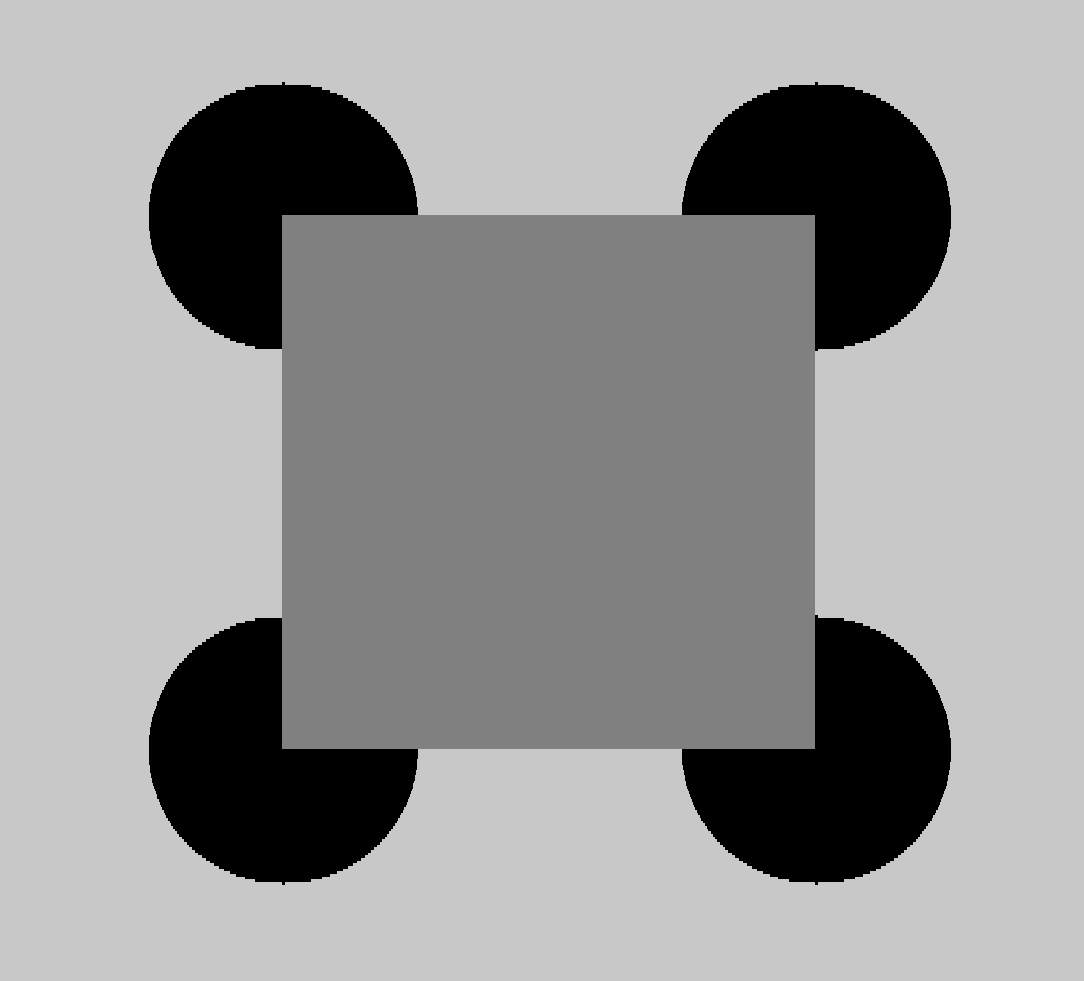
\includegraphics[width=0.4\textwidth,valign=t]{AIKanizsa.png} &
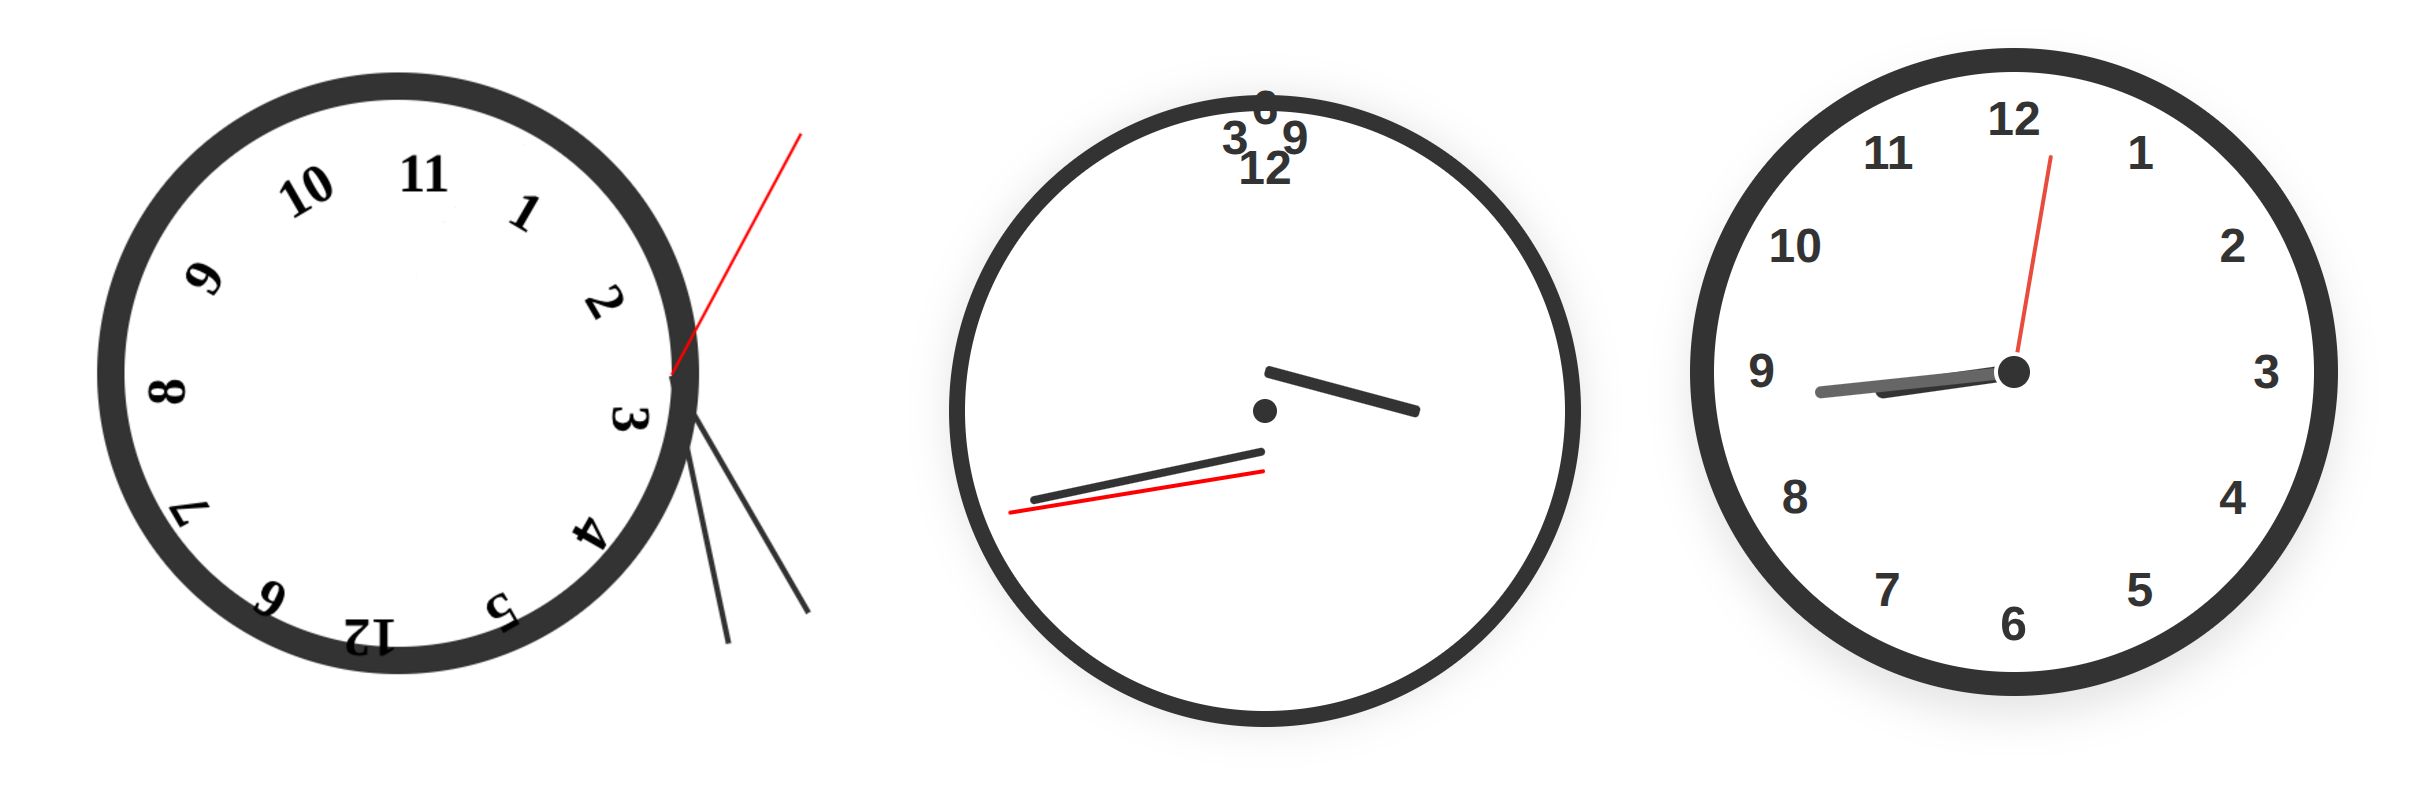
\includegraphics[width=0.6\textwidth,valign=t]{AIclocks.png} \\
\end{tabular}

\caption{\textbf{AI ``blunders'':} Left: Asked by the first author to write a program displaying Kanizsa's illusory rectangle, an AI produced the result above, explaining: ``I have changed the Kanizsa example to make things robust and more visible [...] A darker gray rectangle is drawn at the center, clearly visible against the light-gray background.''. Right: Output from the AI clock project where AIs are asked to write programs drawing a clock; note the correct response on the rigth (See \url{https://clocks.brianmoore.com/} for more).} 
\label{fig:AIBlunders}
\end{figure}

\begin{center}\rule{0.5\linewidth}{0.5pt}\end{center}

\subsection{Author Contributions}\label{author-contributions}

OB\textbf{Christophe Pallier}: Conceptualization, Software implementation, Documentation and Paper Writing, with assistance from \textbf{Claude Sonnet 4.6} and \textbf{Gemini 2.5}. Consistent with current editorial
norms \parencite{natureportfolio2023, springernature2023}, Claude and
Gemini are listed under Author Contributions rather than as a named
author, because authorship requires the capacity to take
accountability for the work.  Christophe Pallier takes full
responsibility for all content.

\textbf{Julie Bonnaire} performed timing tests and redacted a report available in \url{https://github.com/chrplr/goxpyriment/tree/mainperformance-reports}

\textbf{Marie-France Fourcade} designed and built the photodiode system used to measure visual presentation delays in some tests. 

\subsection{Open Practices Statement}\label{open-practices-statement}

The source code of \texttt{goxpyriment} is available under the GNU
General Public License v3 at
https://github.com/chrplr/goxpyriment. All example experiments
described in this article are included in the repository. No empirical
data are reported in this article.

\printbibliography

\newpage
\section*{appendix}

\subsection{Code Availability and Deployment}\label{availability}

\texttt{goxpyriment} is available at \url{https://github.com/chrplr/goxpyriment}
under the GPLv3 license. While the single-binary format simplifies
distribution, users should be aware of modern operating system security
features. 

\textbf{Windows: SmartScreen warning.} When a user downloads a
\texttt{.exe} file from the internet and tries to run it, Windows
Defender SmartScreen may display a ``Windows protected your PC''
warning, because the executable has not been digitally signed.
To proceed the user clicks \textbf{More info} and then
\textbf{Run anyway}. This prompt appears only on first launch and only
for files with the ``downloaded from the internet'' mark of origin; files
copied from a USB drive or an internal network share bypass the check.

\textbf{macOS: Gatekeeper.}
macOS includes a security system called \textbf{Gatekeeper} that checks
whether applications have been signed with an Apple-issued certificate
and submitted to Apple for notarization (a process that requires a paid
Apple Developer account, \$99/year). Applications distributed outside
the Mac App Store that are not notarized receive a quarantine attribute
when downloaded, which triggers Gatekeeper on first launch.

Two dialogs may appear, depending on how the user attempts to open the
application.

\begin{enumerate}
\tightlist
\item \textbf{``App is damaged'' dialog}
  (Figure~\ref{fig:gatekeeper-damaged}).
  This alarming message appears when double-clicking an unsigned
  \texttt{.app} bundle. Despite the wording, the application has not
  been corrupted. \textbf{Workaround:} right-click (or Control-click)
  the \texttt{.app}, choose \textbf{Open} from the contextual menu, then
  click \textbf{Open} in the confirmation dialog. The exception is
  remembered; subsequent double-clicks launch the app normally.

\item \textbf{Privacy \& Security panel}
  (Figure~\ref{fig:gatekeeper-privacy}).
  After a blocked launch attempt, macOS records the blocked app in
  \textbf{System Settings → Privacy \& Security}. Scrolling to the
  blocked-app entry and clicking \textbf{Open Anyway} (followed by the
  administrator password) has the same effect as the right-click method.
\end{enumerate}

For plain command-line binaries (not \texttt{.app} bundles), the
right-click workaround does not apply. Instead, the quarantine attribute
can be removed with:

\begin{verbatim}
xattr -d com.apple.quarantine ./myexperiment
chmod +x ./myexperiment
./myexperiment
\end{verbatim}

\begin{figure}[t]
\centering

\includegraphics[width=0.4\textwidth]{macos-gatekeeper-damaged.png}
\caption{The macOS Gatekeeper ``damaged'' dialog that appears when
double-clicking an unsigned \texttt{.app} bundle downloaded from the
internet. The application is not corrupted; the message reflects the
absence of an Apple notarization certificate. Right-clicking the app
and selecting \emph{Open}, then confirming in the second dialog,
bypasses the restriction permanently for that binary. Note that
sometimes it is also necessary to run a `xttr -d com.apple.quarantine myapp` command
(see text)}
\label{fig:gatekeeper-damaged}
\end{figure}

\begin{figure}[t]
\centering
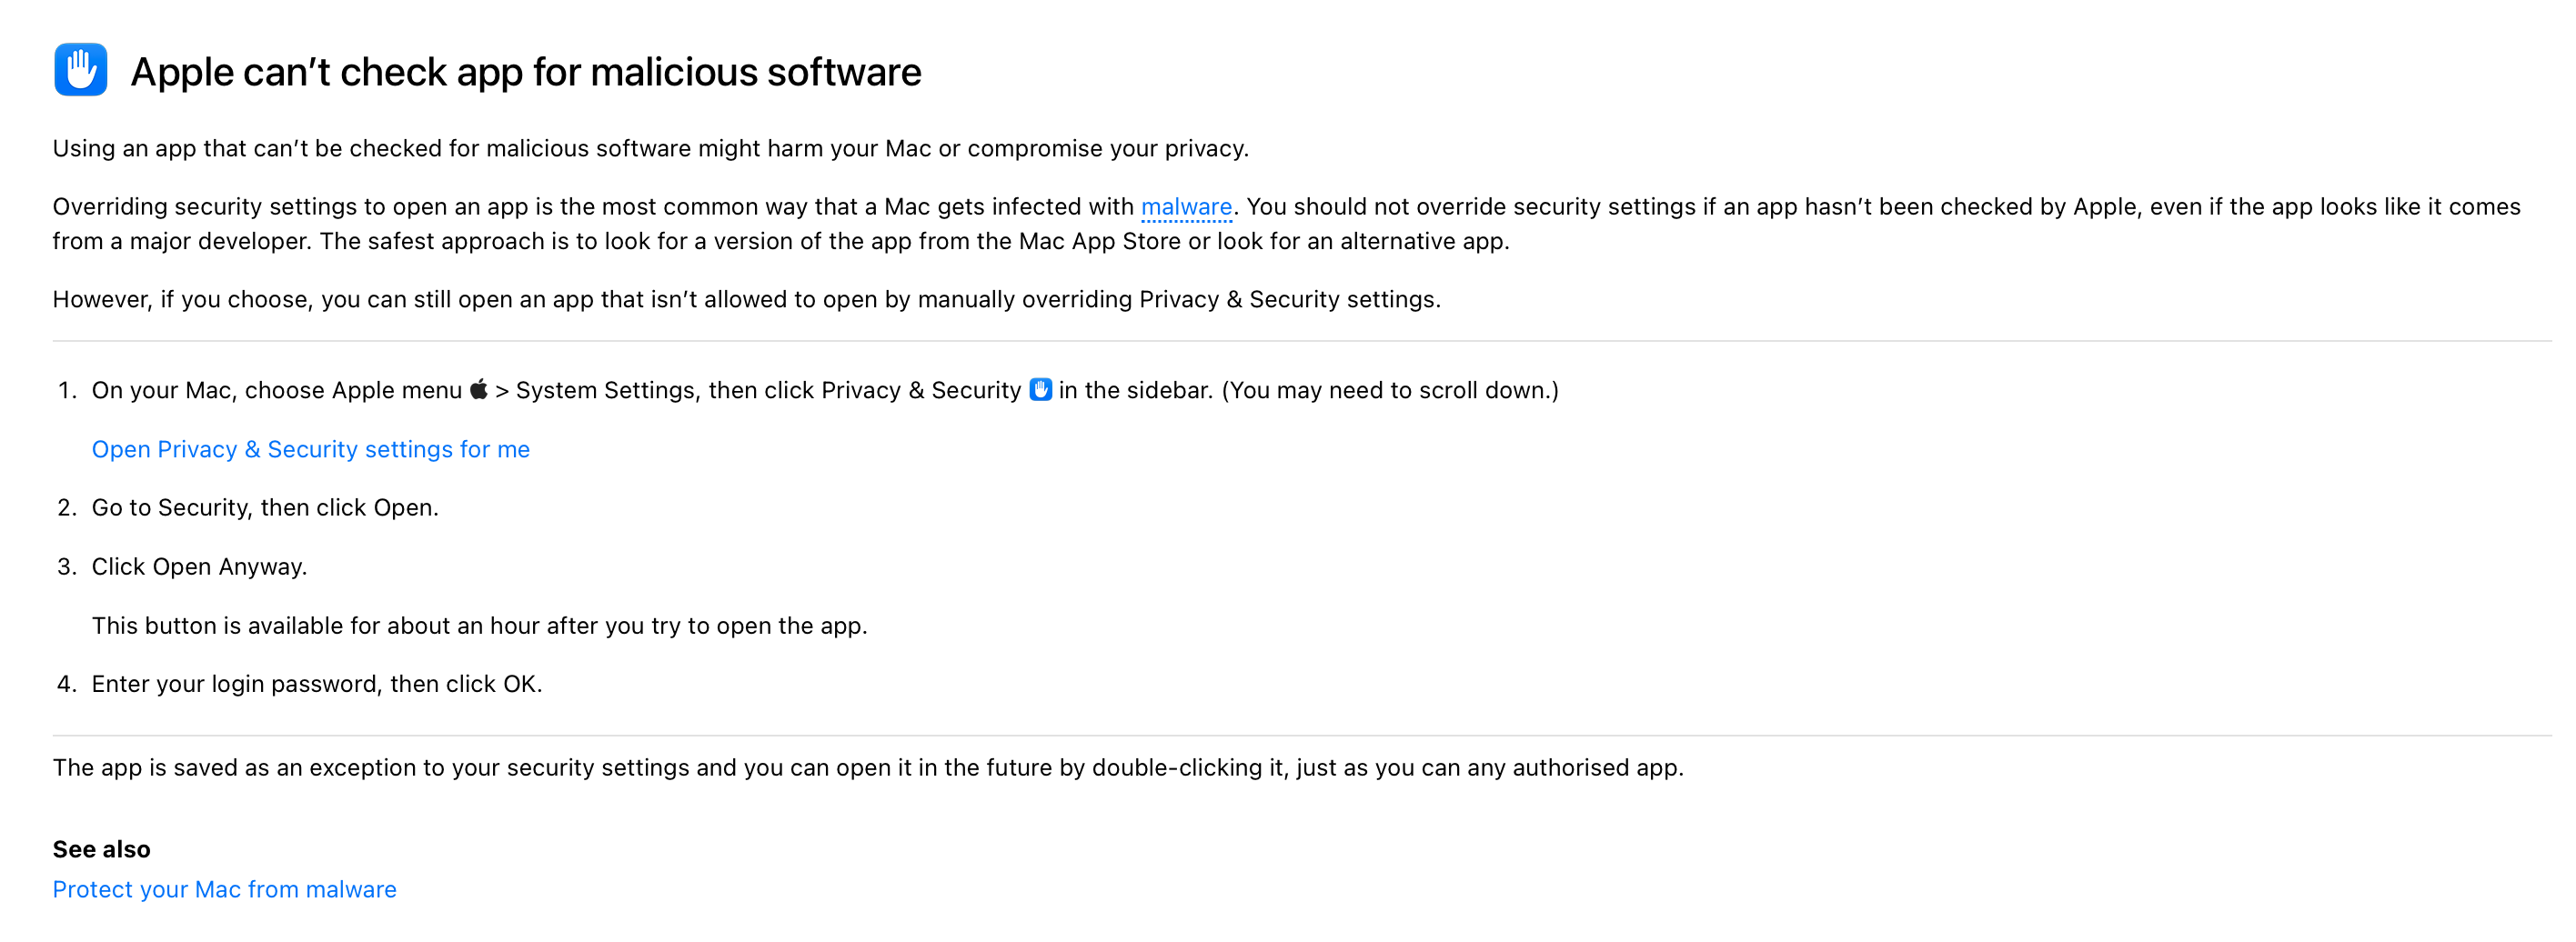
\includegraphics[width=\textwidth]{macos-gatekeeper-privacy.png}
\caption{The Privacy \& Security pane in macOS System Settings showing
a blocked unsigned application. Clicking \emph{Open Anyway} and
supplying the administrator password grants a permanent exception for
that binary.}
\label{fig:gatekeeper-privacy}
\end{figure}

\textbf{Linux.} Linux binaries compiled with \texttt{go build} require
no installation: copy the binary to the target machine, mark it
executable (\texttt{chmod +x}), and run it. For broader distribution,
the AppImage format (\url{https://appimage.org}) encapsulates a binary
and its required shared libraries into a single portable file that runs
on most Linux distributions without root access.


\end{document}
